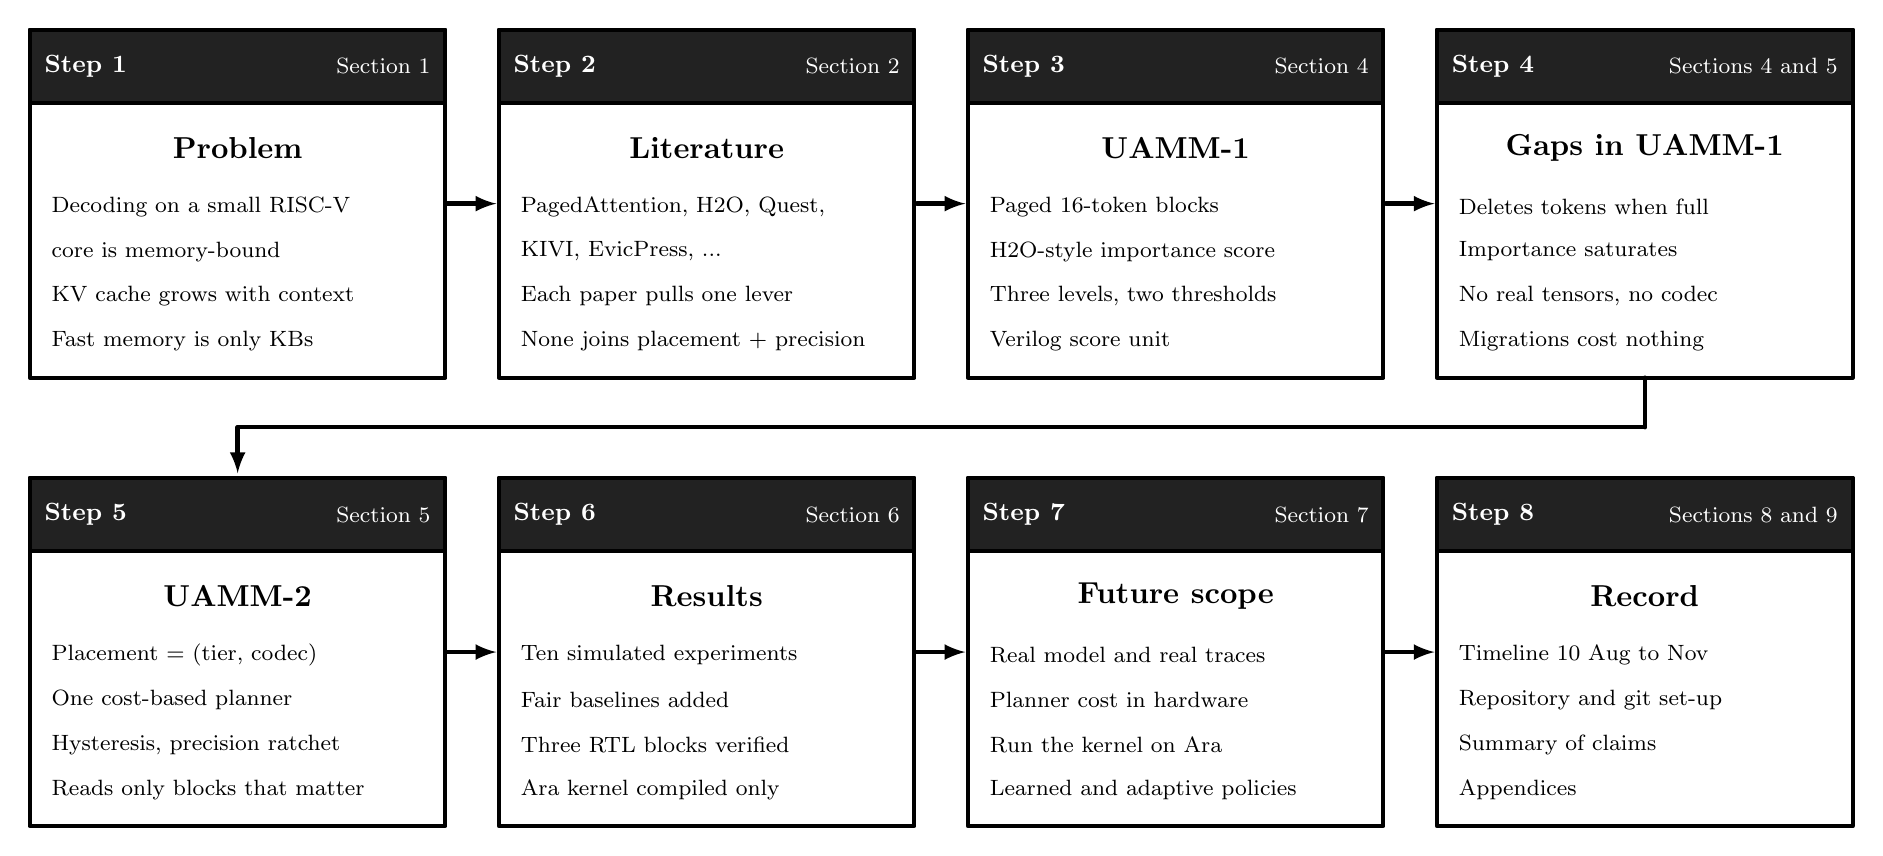
\begin{tikzpicture}[line cap=round,line join=round]
\draw[line width=1.44pt,draw={rgb,255:red,0;green,0;blue,0},fill={rgb,255:red,255;green,255;blue,255}] (0.148in,2.478in) rectangle (2.227in,4.218in);
\draw[line width=1.44pt,draw={rgb,255:red,0;green,0;blue,0},fill={rgb,255:red,34;green,34;blue,34}] (0.148in,3.852in) rectangle (2.227in,4.218in);
\draw[line width=1.44pt,draw={rgb,255:red,0;green,0;blue,0},fill={rgb,255:red,255;green,255;blue,255}] (2.494in,2.478in) rectangle (4.572in,4.218in);
\draw[line width=1.44pt,draw={rgb,255:red,0;green,0;blue,0},fill={rgb,255:red,34;green,34;blue,34}] (2.494in,3.852in) rectangle (4.572in,4.218in);
\draw[line width=1.44pt,draw={rgb,255:red,0;green,0;blue,0},fill={rgb,255:red,255;green,255;blue,255}] (4.839in,2.478in) rectangle (6.917in,4.218in);
\draw[line width=1.44pt,draw={rgb,255:red,0;green,0;blue,0},fill={rgb,255:red,34;green,34;blue,34}] (4.839in,3.852in) rectangle (6.917in,4.218in);
\draw[line width=1.44pt,draw={rgb,255:red,0;green,0;blue,0},fill={rgb,255:red,255;green,255;blue,255}] (7.184in,2.478in) rectangle (9.263in,4.218in);
\draw[line width=1.44pt,draw={rgb,255:red,0;green,0;blue,0},fill={rgb,255:red,34;green,34;blue,34}] (7.184in,3.852in) rectangle (9.263in,4.218in);
\draw[line width=1.44pt,draw={rgb,255:red,0;green,0;blue,0},fill={rgb,255:red,255;green,255;blue,255}] (0.148in,0.236in) rectangle (2.227in,1.976in);
\draw[line width=1.44pt,draw={rgb,255:red,0;green,0;blue,0},fill={rgb,255:red,34;green,34;blue,34}] (0.148in,1.610in) rectangle (2.227in,1.976in);
\draw[line width=1.44pt,draw={rgb,255:red,0;green,0;blue,0},fill={rgb,255:red,255;green,255;blue,255}] (2.494in,0.236in) rectangle (4.572in,1.976in);
\draw[line width=1.44pt,draw={rgb,255:red,0;green,0;blue,0},fill={rgb,255:red,34;green,34;blue,34}] (2.494in,1.610in) rectangle (4.572in,1.976in);
\draw[line width=1.44pt,draw={rgb,255:red,0;green,0;blue,0},fill={rgb,255:red,255;green,255;blue,255}] (4.839in,0.236in) rectangle (6.917in,1.976in);
\draw[line width=1.44pt,draw={rgb,255:red,0;green,0;blue,0},fill={rgb,255:red,34;green,34;blue,34}] (4.839in,1.610in) rectangle (6.917in,1.976in);
\draw[line width=1.44pt,draw={rgb,255:red,0;green,0;blue,0},fill={rgb,255:red,255;green,255;blue,255}] (7.184in,0.236in) rectangle (9.263in,1.976in);
\draw[line width=1.44pt,draw={rgb,255:red,0;green,0;blue,0},fill={rgb,255:red,34;green,34;blue,34}] (7.184in,1.610in) rectangle (9.263in,1.976in);
\draw[line width=1.58pt,draw={rgb,255:red,0;green,0;blue,0}] (8.223in,2.478in) -- (8.223in,2.230in);
\draw[line width=1.58pt,draw={rgb,255:red,0;green,0;blue,0}] (8.223in,2.230in) -- (1.188in,2.230in);
\node[anchor=west,align=left,text={rgb,255:red,255;green,255;blue,255},font=\fontsize{9.2pt}{10.8pt}\selectfont\bfseries,inner sep=0pt] at (0.220in,4.035in) {Step 1};
\node[anchor=east,align=right,text={rgb,255:red,255;green,255;blue,255},font=\fontsize{8.0pt}{9.5pt}\selectfont,inner sep=0pt] at (2.155in,4.035in) {Section 1};
\node[align=center,text={rgb,255:red,0;green,0;blue,0},font=\fontsize{10.7pt}{12.7pt}\selectfont\bfseries,inner sep=0pt] at (1.188in,3.628in) {Problem};
\node[anchor=west,align=left,text={rgb,255:red,0;green,0;blue,0},font=\fontsize{8.0pt}{9.5pt}\selectfont,inner sep=0pt] at (0.255in,3.333in) {Decoding on a small RISC-V};
\node[anchor=west,align=left,text={rgb,255:red,0;green,0;blue,0},font=\fontsize{8.0pt}{9.5pt}\selectfont,inner sep=0pt] at (0.255in,3.109in) {core is memory-bound};
\node[anchor=west,align=left,text={rgb,255:red,0;green,0;blue,0},font=\fontsize{8.0pt}{9.5pt}\selectfont,inner sep=0pt] at (0.255in,2.885in) {KV cache grows with context};
\node[anchor=west,align=left,text={rgb,255:red,0;green,0;blue,0},font=\fontsize{8.0pt}{9.5pt}\selectfont,inner sep=0pt] at (0.255in,2.661in) {Fast memory is only KBs};
\node[anchor=west,align=left,text={rgb,255:red,255;green,255;blue,255},font=\fontsize{9.2pt}{10.8pt}\selectfont\bfseries,inner sep=0pt] at (2.565in,4.035in) {Step 2};
\node[anchor=east,align=right,text={rgb,255:red,255;green,255;blue,255},font=\fontsize{8.0pt}{9.5pt}\selectfont,inner sep=0pt] at (4.501in,4.035in) {Section 2};
\node[align=center,text={rgb,255:red,0;green,0;blue,0},font=\fontsize{10.7pt}{12.7pt}\selectfont\bfseries,inner sep=0pt] at (3.533in,3.628in) {Literature};
\node[anchor=west,align=left,text={rgb,255:red,0;green,0;blue,0},font=\fontsize{8.0pt}{9.5pt}\selectfont,inner sep=0pt] at (2.601in,3.333in) {PagedAttention, H2O, Quest,};
\node[anchor=west,align=left,text={rgb,255:red,0;green,0;blue,0},font=\fontsize{8.0pt}{9.5pt}\selectfont,inner sep=0pt] at (2.601in,3.109in) {KIVI, EvicPress, ...};
\node[anchor=west,align=left,text={rgb,255:red,0;green,0;blue,0},font=\fontsize{8.0pt}{9.5pt}\selectfont,inner sep=0pt] at (2.601in,2.885in) {Each paper pulls one lever};
\node[anchor=west,align=left,text={rgb,255:red,0;green,0;blue,0},font=\fontsize{8.0pt}{9.5pt}\selectfont,inner sep=0pt] at (2.601in,2.661in) {None joins placement + precision};
\node[anchor=west,align=left,text={rgb,255:red,255;green,255;blue,255},font=\fontsize{9.2pt}{10.8pt}\selectfont\bfseries,inner sep=0pt] at (4.910in,4.035in) {Step 3};
\node[anchor=east,align=right,text={rgb,255:red,255;green,255;blue,255},font=\fontsize{8.0pt}{9.5pt}\selectfont,inner sep=0pt] at (6.846in,4.035in) {Section 4};
\node[align=center,text={rgb,255:red,0;green,0;blue,0},font=\fontsize{10.7pt}{12.7pt}\selectfont\bfseries,inner sep=0pt] at (5.878in,3.628in) {UAMM-1};
\node[anchor=west,align=left,text={rgb,255:red,0;green,0;blue,0},font=\fontsize{8.0pt}{9.5pt}\selectfont,inner sep=0pt] at (4.946in,3.333in) {Paged 16-token blocks};
\node[anchor=west,align=left,text={rgb,255:red,0;green,0;blue,0},font=\fontsize{8.0pt}{9.5pt}\selectfont,inner sep=0pt] at (4.946in,3.109in) {H2O-style importance score};
\node[anchor=west,align=left,text={rgb,255:red,0;green,0;blue,0},font=\fontsize{8.0pt}{9.5pt}\selectfont,inner sep=0pt] at (4.946in,2.885in) {Three levels, two thresholds};
\node[anchor=west,align=left,text={rgb,255:red,0;green,0;blue,0},font=\fontsize{8.0pt}{9.5pt}\selectfont,inner sep=0pt] at (4.946in,2.661in) {Verilog score unit};
\node[anchor=west,align=left,text={rgb,255:red,255;green,255;blue,255},font=\fontsize{9.2pt}{10.8pt}\selectfont\bfseries,inner sep=0pt] at (7.256in,4.035in) {Step 4};
\node[anchor=east,align=right,text={rgb,255:red,255;green,255;blue,255},font=\fontsize{8.0pt}{9.5pt}\selectfont,inner sep=0pt] at (9.191in,4.035in) {Sections 4 and 5};
\node[align=center,text={rgb,255:red,0;green,0;blue,0},font=\fontsize{10.7pt}{12.7pt}\selectfont\bfseries,inner sep=0pt] at (8.223in,3.628in) {Gaps in UAMM-1};
\node[anchor=west,align=left,text={rgb,255:red,0;green,0;blue,0},font=\fontsize{8.0pt}{9.5pt}\selectfont,inner sep=0pt] at (7.291in,3.333in) {Deletes tokens when full};
\node[anchor=west,align=left,text={rgb,255:red,0;green,0;blue,0},font=\fontsize{8.0pt}{9.5pt}\selectfont,inner sep=0pt] at (7.291in,3.109in) {Importance saturates};
\node[anchor=west,align=left,text={rgb,255:red,0;green,0;blue,0},font=\fontsize{8.0pt}{9.5pt}\selectfont,inner sep=0pt] at (7.291in,2.885in) {No real tensors, no codec};
\node[anchor=west,align=left,text={rgb,255:red,0;green,0;blue,0},font=\fontsize{8.0pt}{9.5pt}\selectfont,inner sep=0pt] at (7.291in,2.661in) {Migrations cost nothing};
\node[anchor=west,align=left,text={rgb,255:red,255;green,255;blue,255},font=\fontsize{9.2pt}{10.8pt}\selectfont\bfseries,inner sep=0pt] at (0.220in,1.793in) {Step 5};
\node[anchor=east,align=right,text={rgb,255:red,255;green,255;blue,255},font=\fontsize{8.0pt}{9.5pt}\selectfont,inner sep=0pt] at (2.155in,1.793in) {Section 5};
\node[align=center,text={rgb,255:red,0;green,0;blue,0},font=\fontsize{10.7pt}{12.7pt}\selectfont\bfseries,inner sep=0pt] at (1.188in,1.386in) {UAMM-2};
\node[anchor=west,align=left,text={rgb,255:red,0;green,0;blue,0},font=\fontsize{8.0pt}{9.5pt}\selectfont,inner sep=0pt] at (0.255in,1.091in) {Placement = (tier, codec)};
\node[anchor=west,align=left,text={rgb,255:red,0;green,0;blue,0},font=\fontsize{8.0pt}{9.5pt}\selectfont,inner sep=0pt] at (0.255in,0.867in) {One cost-based planner};
\node[anchor=west,align=left,text={rgb,255:red,0;green,0;blue,0},font=\fontsize{8.0pt}{9.5pt}\selectfont,inner sep=0pt] at (0.255in,0.643in) {Hysteresis, precision ratchet};
\node[anchor=west,align=left,text={rgb,255:red,0;green,0;blue,0},font=\fontsize{8.0pt}{9.5pt}\selectfont,inner sep=0pt] at (0.255in,0.419in) {Reads only blocks that matter};
\node[anchor=west,align=left,text={rgb,255:red,255;green,255;blue,255},font=\fontsize{9.2pt}{10.8pt}\selectfont\bfseries,inner sep=0pt] at (2.565in,1.793in) {Step 6};
\node[anchor=east,align=right,text={rgb,255:red,255;green,255;blue,255},font=\fontsize{8.0pt}{9.5pt}\selectfont,inner sep=0pt] at (4.501in,1.793in) {Section 6};
\node[align=center,text={rgb,255:red,0;green,0;blue,0},font=\fontsize{10.7pt}{12.7pt}\selectfont\bfseries,inner sep=0pt] at (3.533in,1.386in) {Results};
\node[anchor=west,align=left,text={rgb,255:red,0;green,0;blue,0},font=\fontsize{8.0pt}{9.5pt}\selectfont,inner sep=0pt] at (2.601in,1.091in) {Ten simulated experiments};
\node[anchor=west,align=left,text={rgb,255:red,0;green,0;blue,0},font=\fontsize{8.0pt}{9.5pt}\selectfont,inner sep=0pt] at (2.601in,0.867in) {Fair baselines added};
\node[anchor=west,align=left,text={rgb,255:red,0;green,0;blue,0},font=\fontsize{8.0pt}{9.5pt}\selectfont,inner sep=0pt] at (2.601in,0.643in) {Three RTL blocks verified};
\node[anchor=west,align=left,text={rgb,255:red,0;green,0;blue,0},font=\fontsize{8.0pt}{9.5pt}\selectfont,inner sep=0pt] at (2.601in,0.419in) {Ara kernel compiled only};
\node[anchor=west,align=left,text={rgb,255:red,255;green,255;blue,255},font=\fontsize{9.2pt}{10.8pt}\selectfont\bfseries,inner sep=0pt] at (4.910in,1.793in) {Step 7};
\node[anchor=east,align=right,text={rgb,255:red,255;green,255;blue,255},font=\fontsize{8.0pt}{9.5pt}\selectfont,inner sep=0pt] at (6.846in,1.793in) {Section 7};
\node[align=center,text={rgb,255:red,0;green,0;blue,0},font=\fontsize{10.7pt}{12.7pt}\selectfont\bfseries,inner sep=0pt] at (5.878in,1.386in) {Future scope};
\node[anchor=west,align=left,text={rgb,255:red,0;green,0;blue,0},font=\fontsize{8.0pt}{9.5pt}\selectfont,inner sep=0pt] at (4.946in,1.091in) {Real model and real traces};
\node[anchor=west,align=left,text={rgb,255:red,0;green,0;blue,0},font=\fontsize{8.0pt}{9.5pt}\selectfont,inner sep=0pt] at (4.946in,0.867in) {Planner cost in hardware};
\node[anchor=west,align=left,text={rgb,255:red,0;green,0;blue,0},font=\fontsize{8.0pt}{9.5pt}\selectfont,inner sep=0pt] at (4.946in,0.643in) {Run the kernel on Ara};
\node[anchor=west,align=left,text={rgb,255:red,0;green,0;blue,0},font=\fontsize{8.0pt}{9.5pt}\selectfont,inner sep=0pt] at (4.946in,0.419in) {Learned and adaptive policies};
\node[anchor=west,align=left,text={rgb,255:red,255;green,255;blue,255},font=\fontsize{9.2pt}{10.8pt}\selectfont\bfseries,inner sep=0pt] at (7.256in,1.793in) {Step 8};
\node[anchor=east,align=right,text={rgb,255:red,255;green,255;blue,255},font=\fontsize{8.0pt}{9.5pt}\selectfont,inner sep=0pt] at (9.191in,1.793in) {Sections 8 and 9};
\node[align=center,text={rgb,255:red,0;green,0;blue,0},font=\fontsize{10.7pt}{12.7pt}\selectfont\bfseries,inner sep=0pt] at (8.223in,1.386in) {Record};
\node[anchor=west,align=left,text={rgb,255:red,0;green,0;blue,0},font=\fontsize{8.0pt}{9.5pt}\selectfont,inner sep=0pt] at (7.291in,1.091in) {Timeline 10 Aug to Nov};
\node[anchor=west,align=left,text={rgb,255:red,0;green,0;blue,0},font=\fontsize{8.0pt}{9.5pt}\selectfont,inner sep=0pt] at (7.291in,0.867in) {Repository and git set-up};
\node[anchor=west,align=left,text={rgb,255:red,0;green,0;blue,0},font=\fontsize{8.0pt}{9.5pt}\selectfont,inner sep=0pt] at (7.291in,0.643in) {Summary of claims};
\node[anchor=west,align=left,text={rgb,255:red,0;green,0;blue,0},font=\fontsize{8.0pt}{9.5pt}\selectfont,inner sep=0pt] at (7.291in,0.419in) {Appendices};
\draw[-latex,line width=1.58pt,draw={rgb,255:red,0;green,0;blue,0}] (2.238in,3.348in) -- (2.482in,3.348in);
\draw[-latex,line width=1.58pt,draw={rgb,255:red,0;green,0;blue,0}] (4.584in,3.348in) -- (4.827in,3.348in);
\draw[-latex,line width=1.58pt,draw={rgb,255:red,0;green,0;blue,0}] (6.929in,3.348in) -- (7.173in,3.348in);
\draw[-latex,line width=1.58pt,draw={rgb,255:red,0;green,0;blue,0}] (1.188in,2.230in) -- (1.188in,2.000in);
\draw[-latex,line width=1.58pt,draw={rgb,255:red,0;green,0;blue,0}] (2.238in,1.106in) -- (2.482in,1.106in);
\draw[-latex,line width=1.58pt,draw={rgb,255:red,0;green,0;blue,0}] (4.584in,1.106in) -- (4.827in,1.106in);
\draw[-latex,line width=1.58pt,draw={rgb,255:red,0;green,0;blue,0}] (6.929in,1.106in) -- (7.173in,1.106in);
\end{tikzpicture}
